\documentclass{sig-alternate}

\setcopyright{acmcopyright}
\usepackage{amsmath}
\usepackage{amssymb}
\usepackage{framed}
\usepackage{url}
%\usepackage[disable]{todonotes}
\usepackage{todonotes}
\usepackage{graphicx}
\usepackage{float}
\usepackage{tabularx}
\usepackage{fancyvrb}

\renewcommand{\textfraction}{0.05}
\renewcommand{\topfraction}{0.9}
\renewcommand{\bottomfraction}{0.9}
\renewcommand{\floatpagefraction}{0.75}

%-----------------------------------------------------------------
%-----------------------------------------------------------------
\begin{document}
%-----------------------------------------------------------------
%-----------------------------------------------------------------

\title{Nipping Bugs in the Bud\\ Student Mistakes in Introductory Computer Science}
\numberofauthors{3}
\author{
\alignauthor
%Nivedita Chopra\\
%       \affaddr{Carnegie Mellon University}\\
%      \affaddr{Pittsburgh, PA}\\
%     \email{niveditc@andrew.cmu.edu}
%     \additionalauthors{Additional authors: Robert Simmons (Carnegie Mellon University,
%email: {\texttt{rjsimmon@cs.cmu.edu}}) and Roy Maxion
%(Carnegie Mellon University, email: {\texttt{maxion@cs.cmu.edu}}).}
}
%\date{\today}
\maketitle

\presetkeys{todonotes}{color=red!30}{}
% TODO : Remove page numbers before submission
\setcounter{page}{1}
\pagenumbering{arabic}

% IEEE bug counts
\def\numlogicIEEE{64 }
\def\numdataIEEE{30 }
\def\numinterfaceIEEE{5 }
\def\numotherIEEE{27 }

% Final bug counts
\def\numlogic{61 }
\def\numdata{27 }
\def\numinterface{5 }
\def\numcomp{33 }
\def\numtotal{126 }
\def\numedge{31 }

\begin{abstract}

Bugs in computer programs are often caused by mistakes in the
programmer's thought process. Diagnosing such bugs in student code in
introductory computer science classes takes a great deal of time and
effort for both the students and the course staff. We aim to provide a
description of the kinds of bugs that are seen in introductory
computer science classes, which will help instructors formulate plans
to better prepare students for dealing with these errors. We collected
information about bugs committed by students, including a description
of the bug, an optional code snippet, and the student's reasoning
behind the bug. We then classified each bug according to a standard
taxonomy (IEEE Standard Classification of Software Anomalies (2010))
and determined the mistakes behind common bugs. We found \numlogic
logic bugs, \numdata data bugs, and \numinterface interface bugs per
the IEEE standard. An additional category of bugs emerged that we
called ``comprehension errors'' (\numcomp instances), which may be
unique to introductory computer science classes. Comprehension errors
are caused by a misunderstanding of concepts, specifications, or error
messages, and so classifying bugs using this category may prove useful
in highlighting concepts that need to be explained better. We believe
that our taxonomy is generally applicable to introductory computer
science courses and can form a basis for a formal discussion of bugs
seen in these classes.

\end{abstract}

%-----------------------------------------------------------------
\section{Introduction}
\label{sec:intro}
%-----------------------------------------------------------------

Bugs are a major problem in all areas of software development, and it
is no surprise that they are also a big problem for students in
introductory computer science courses. Even students who learn
relatively quickly to detect and fix errors in syntax may have trouble
detecting and fixing bugs caused by mistakes in their thought
processes.  For example, a student who has misunderstood the workings
of pointer arithmetic may add the wrong quantity to a pointer, causing
memory corruption that is difficult to understand and diagnose.\\

Diagnosing and correcting bugs in student code takes a significant
amount of time and effort by both students and the course staff. In
our experience with large introductory computer science classes, we
have found that both students and the course staff lack a common and
formal language for talking about the kinds of bugs that are seen in
student code during office hours and labs. This makes it difficult to
assess the kinds of errors that students are unable to self-diagnose
and to formulate plans for better preparing students to deal with such
errors.\\

Our approach is to catalog the bugs committed by students in an
introductory computer science class. Initially, we sought to use a
standard taxonomy of software bugs \cite{IEEE10} to classify the bugs
that were recorded. Eventually, we modified this taxonomy based on our
semester-long observation of student bugs. We present our observations
and modified taxonomy, which we believe is generally applicable to
introductory computer science courses.

%-----------------------------------------------------------------
\section{Background and related work}
\label{sec:background}
%-----------------------------------------------------------------

In the 1980s, much research was aimed at examining bugs committed by
students learning to program, and determining flaws in student
reasoning from a cognitive standpoint
\cite{JoniSolowayGoldmanEhrlich83, Pea86, PutnamSleemanBaxterKuspa86,
SpohrerSoloway86}. Much of this work was focused on the student's
understanding of specific language constructs such as loops,
conditional statements, arrays, etc.
\cite{JoniSolowayGoldmanEhrlich83, Pea86, PutnamSleemanBaxterKuspa86}.
An example illustrating this is a student misunderstanding of the
semantics of a while loop, and making the assumption that the loop
condition is being checked at every point within the loop body and not
just at the beginning of each iteration of the loop \cite{Pea86}.\\

Most of the work done in the 1980s focused on novice programmers who
were learning to program for the first time
\cite{Pea86,SpohrerSoloway86}. Our research focuses on students who
already know how to program, having taken at least one semester-long
programming class. Thus we focus on the students' understanding of
algorithms and data structures, and other concepts they are learning
for the first time. We also classify the bugs committed by students in
the class in a broader sense and avoid focusing on details that are
specific to our class and the language in which it is taught
\cite{Arnold10}.\\

%-----------------------------------------------------------------
\begin{table*}[t]
\def\arraystretch{1.6}
\centering
\caption{Error classification by type as per the IEEE Standard Classification for Software Anomalies \cite{IEEE10}}
\label{table:IEEE}
\begin{tabular}{|p{1in}|p{2.9in}|p{2.6in}|} \hline
\textbf{Type} & \textbf{Description} & \textbf{Example}\\ \hline
Data Error&
Defect in data definition, initialization, mapping, access or use.&
Failure to initialize a variable, modifying data structures in non-destructive operations, etc.\\ \hline

Logic Error&
Defect in decision logic, branching, sequencing, or computational algorithm.&
Incorrect sequencing of code statements, missing cases, performing the wrong operation, etc.\\ \hline

Interface Error&
Defect in specification or implementation of an interface (e.g., between user and machine, between two software modules, etc.)&
Use of implementation functions in client code, writing an implementation that does not conform to the interface, etc.\\ \hline

Syntax Error&
Nonconformity with the defined rules of a language.&
Missing semicolon, mismatched braces, etc.\\ \hline

Description Error&
Defect in description of software or its use, installation, or operation.&
\\ \hline

Standards Error&
Nonconformity with a defined standard.&
\\ \hline

Other Error&
Defect with no defined type.
&
\\ \hline
\end{tabular}
\end{table*}
%-----------------------------------------------------------------

Ko and Myers' work \cite{KoMyers03} classifies and describes errors in
programming by linking the errors to their causes. Their model for
programming errors is based on Reason's model \cite{Reason90}.
Reason's model demonstrates that mistakes in applying knowledge and
strategy cause the cognitive problems that lead to errors. Ko and
Myers provide a broad taxonomy for errors seen in all types of
programming, including both industry and education. Ko and Myers share
our goal of connecting errors in programming to mistakes in the
programmer's thought process. However, our research focuses on
introductory programming classes, and we provide a taxonomy tailored
for that purpose.\vspace{8pt}

Recently, Bryce et al. studied bugs in introductory computer science
classes to examine the problems that students face in these classes
with the aim of alleviating student frustration and attrition
\cite{BryceCooleyHansenHayrapetyan10}. They followed a method similar
to ours, of asking students to fill in a form reporting their bugs,
yet they differ from our research in two important aspects. First,
their classification of bugs is very detailed, with 20 disjoint
categories, and focuses heavily on particular concepts and ideas
covered in the class, so it is not applicable beyond their class
unless changes are made.  Second, they do not examine student
reasoning behind the bug; they classify bugs based entirely on the
description and code for the bug.\vspace{8pt}

For the purposes of our research, we distinguished between bugs, which
are errors based on flawed knowledge, and slips, which are errors
based on ``random noise'' \cite{VanLehn90}. While programming, slips
are usually manifested as syntax errors and some other errors that may
cause a program to fail compilation. On the other hand, bugs are
caused by mistakes in the programmer's thought process. In our
research, we consider only bugs and we ignore slips entirely. This is
because slips in programming may be self-correcting, since they almost
always cause compile errors which may be easily fixed by the
programmer.\vspace{8pt}

Our research was performed in an introductory computer science class,
taught in a small safe subset of the C programming language
\cite{Arnold10}, and in C. The class introduces computer science
students to basic algorithms such as searching and sorting, data
structures such as lists, stacks, queues, heaps, trees, etc. and
computational ideas such as complexity analysis and proof of
correctness of code.


%-----------------------------------------------------------------
\section{Method}
\label{sec:method}
%-----------------------------------------------------------------

We recorded bugs committed by the students taking the class in Fall
2014. Each record of data contained a description of the bug, an
optional snippet of the buggy code, and a short explanation by the
student of the cause behind the committing of the bug. An example of a
record of data is shown in Figure \ref{fig:record}.\\

%-----------------------------------------------------------------
\begin{figure}
\begin{framed}
\emph{What was the bug?}\\
\verb|NULL| pointer dereference\\

\emph{What caused you to write buggy code?}\\
 I did not think of edge cases while writing the code\\

\emph{Include a snippet of the buggy code (optional)}\\
\verb|list = list->next;| //where \verb|list| is \verb|NULL|
\end{framed}
\vspace{-0.1in}
\caption{Example of a record of data}
\label{fig:record}
\end{figure}
%-----------------------------------------------------------------

Bugs were obtained and recorded in the following ways:
\begin{itemize}

\item{\textbf{Google form.} Students were asked to fill an online form
when they found and fixed a bug. In addition to the data points
mentioned above, data from this source also contained information on
how much time it took the student to find and fix their bug, how they
found the bug, and suggestions for things the course staff may have
done to prevent them from committing the bug or to help them fix it
faster.}

\item{\textbf{Student observation.} We observed students in labs and
office hours, and took note of the bugs committed by students in those
settings. When students fixed their bugs, usually with our help, we
asked them to explain their bug and their reasoning behind what caused
them to commit the bug.}

\item{\textbf{Piazza.} We analyzed posts made in the online Q\&A
forum, Piazza, and recorded the bugs seen there. These posts included
a description and/or code pertaining to the bug, and a discussion that
led to the bug being solved. Some of the data from this source did not
contain student reasoning behind the bug.}

\end{itemize}

With a view towards further examining these bugs, we classified them
according to the IEEE Standard Classification for Software Anomalies.
This document provides a standard for classifying anomalies seen
during software development. It enables organizations to get insight
into the bugs seen during their software development process. The IEEE
standard classifies software anomalies seen in production code on the
basis of attributes such as type, severity, probability, effect, etc.
For the purposes of our research, we only care about the
classification based on type, as outlined in Table \ref{table:IEEE}.
\cite{IEEE10}.\\

When we classified the collected bugs according to the IEEE standard,
we noticed that bugs fell into the logic error (\numlogicIEEE
instances), data error (\numdataIEEE instances) and interface error
(\numinterfaceIEEE instances) categories. \numotherIEEE instances were
categorized as other errors, with no defined type. Three logic errors
and three data errors were later reclassified as comprehension errors
(Section \ref{sec:comprehension}).\\

%-----------------------------------------------------------------
\begin{figure}
\begin{framed}
\setlength{\parindent}{0cm}
\textbf{Problem}\\
Create the list containing 1, 2, and 4, in order, using the \texttt{cons} and \texttt{nil} functions.\\

\texttt{list cons(int, list); /* Adds the integer to the beginning of the list */\\ list nil(); /* Creates a new empty list */}\\

\textbf{Buggy student solution}\\
\texttt{list L = cons(1, cons(2, cons(4)));}\\

\textbf{Correct solution}\\
\texttt{list L = cons(1, cons(2, cons(4, nil())));}\\

\textbf{Comprehension error}\\
Misunderstanding the specification of \texttt{cons} and \texttt{nil}.
\end{framed}
\vspace{-0.1in}
\caption{Comprehension error due to misunderstanding specifications}
\label{fig:comp1}
\end{figure}
%-----------------------------------------------------------------


None of our bugs fell into the other three categories of the IEEE
standard --- syntax error, description error and standards error. As
explained in Section \ref{sec:background}, syntax errors are slips by
the programmer, and not bugs, hence they do not appear in our taxonomy
of bugs. We do not encounter description errors because we operate
under the assumption that the specification provided to students does
not contain errors, since it has been thoroughly playtested by the
course staff. Additionally, we do not deal with standards, hence
standard error is irrelevant.\\

By examining the reasoning provided by students, we realized that we
could classify all the bugs that fell into the ``other'' error
category of the IEEE standard as ``comprehension errors,'' which are
described in the next section.

%-----------------------------------------------------------------
\newpage
\section{Comprehension Errors}
\label{sec:comprehension}
%-----------------------------------------------------------------

While classifying bugs seen in our research, we developed a new
category of bugs that is not described by the IEEE classification. We
call this new category ``comprehension errors,'' and we feel that it
may be unique, or at least particularly relevant, to introductory
computer science classes.\\

A comprehension error occurs when the bug committed by a student is
caused by a misunderstanding on the student's part. Examining student
reasoning behind a bug is the best way to determine whether the bug is
the result of a comprehension error.\\

To better explain the nature of comprehension errors, we highlight
three subcategories of comprehension errors: lacking clarity in a
concept, misunderstanding specifications, and misunderstanding error
messages. This subcategorization is a work in progress, and the
categories are neither exhaustive nor necessarily mutually orthogonal.

%-------------------------------------------
\subsection{Misunderstanding specifications}
\label{sec:comp1}
%-------------------------------------------

Students are often unfamiliar with reading specifications, and are
hence likely to misunderstand them and to make incorrect assumptions
while programming. Additionally, they may not understand how to use
functions that are provided to help them with generating test cases
for their code. Figure \ref{fig:comp1} illustrates a comprehension
error that is caused by a misunderstanding of the specifications.

%-----------------------------------------------------------------
\begin{figure}
\begin{framed}
\setlength{\parindent}{0cm}
\textbf{Problem}\\

Compute the offset as a signed 16 bit integer that is given as a
two-byte operand to the instruction. Instructions are stored in an
array of (unsigned) bytes (\verb|ubyte *P|) \\

\textbf{Buggy student solution}
\vspace{-0.05in}
\begin{verbatim}
 int16_t o1 = (int16_t)(int8_t)P[pc+1];
 int16_t o2 = (int16_t)(int8_t)P[pc+2];
 int16_t offset = ((o1 << 8) | o2);
\end{verbatim}

\textbf{Correct solution}
\vspace{-0.05in}
\begin{verbatim}
 int16_t o1 = (int16_t)(int8_t)P[pc+1];
 int16_t o2 = (int16_t)(uint16_t)P[pc+2];
 int16_t offset = ((o1 << 8) | o2);
\end{verbatim}

\textbf{Comprehension error}\\

Casts both \verb|o1| and \verb|o2| into signed integers to make
resultant offset signed. Sign extension on \verb|o2| may alter the
final quantity. This shows a misunderstanding of the concept of sign
extension.

\end{framed}
\vspace{-0.1in}
\caption{Comprehension error due to lack of clarity on the concept of sign extension}
\label{fig:comp2}

\end{figure}
%-----------------------------------------------------------------


%----------------------------------------
\subsection{Lacking clarity on a concept}
\label{sec:comp2}
%----------------------------------------

Often students may not fully grasp certain aspects of computer science
concepts, especially those that they have recently learned. They may
misunderstand the use cases of certain algorithms and paradigms,
leading to bugs such as searching for an element in an unsorted array
using binary search (which works only on sorted arrays). Figure
\ref{fig:comp2} illustrates a comprehension error that was caused by
lack of clarity on a concept.




%-------------------------------------------
\subsection{Misunderstanding error messages}
%-------------------------------------------

Due to having limited prior programming experience and possibly
because they are using new tools, students are often stumped by error
messages and warnings, from the compiler and the
autograder\footnote{In this class we grade student code using an
online automatic grading program called Autolab}. Figure
\ref{fig:comp3} illustrates a comprehension error that is caused by
misunderstanding an error message.


%-----------------------------------------------------------------
\begin{figure}
\begin{framed}
\setlength{\parindent}{0cm}
\textbf{Problem} \\
Perform the bitwise AND operation on two integers \texttt{x} and \texttt{y}.\\

\textbf{Buggy student solution} \\
\verb|int z  = x && y|\\

\textbf{Error message}\\
\texttt{:error: type mismatch expected bool found int}\\

\textbf{Student's attempted fix}\\
\verb|bool z = x && y|\\

\textbf{Correct solution}\\
\verb|int z = x & y|\\

\textbf{Comprehension error}\\

Upon reading the error message, the student thinks that \texttt{x} and
\texttt{y} should be Booleans rather than integers. They fail to
realize that this error message can also indicate a problem with the
operator rather than the operands.

\end{framed}
\vspace{-0.1in}
\caption{Comprehension error due to misunderstanding an error message}
\label{fig:comp3}
\end{figure}
%-----------------------------------------------------------------


%-----------------------------------------------------------------
\section{Analysis}
\label{sec:analysis}
%-----------------------------------------------------------------

Our analysis of bugs that were not well classified under the original
IEEE Standard Classification for Software Anomalies led us to create a
new category of ``comprehension error'' (Section
\ref{sec:comprehension}). Several bugs that we had initially
classified as logic and data bugs were better classified by this new
category. Over the course of the semester we observed \numlogic logic
bugs, \numdata data bugs, \numinterface interface bugs, and \numcomp
comprehension errors. Examples of these bugs can be seen in Table
\ref{table:new-taxonomy}.\\




For the bugs that were frequently observed every week, we sought the
student misconceptions that may have led to each bug. Since we
possessed a timestamp for each bug recorded, we could pinpoint the
context in which the bug was made, based on the material covered and
assignments due at that time. The reasoning provided by the
student, as described in the data collection process in Section
\ref{sec:method}, often gave us an insight into the misconception that
caused them to commit that bug. Where the student reasoning behind a
bug was unclear, or where we didn't possess a record of student
reasoning, we employed the method of ``just-so stories,''
\cite{JoniSolowayGoldmanEhrlich83} which tries to reconstruct the
thought process that may have led to a particular bug, and provides a
convincing hypothesis about the student misconception that led to a
particular bug. It is worth highlighting the dangers of using the
``just-so'' method to determine student misconceptions from their
code. Multiple chains of reasoning may lead to the same bug, as
highlighted in Figure \ref{fig:incorrect}, and this may cause the bug
to be classified incorrectly.\\


%-----------------------------------------------------------------
\begin{figure}
\begin{framed}
\setlength{\parindent}{0cm}
\textbf{Problem}\\
Write a function to check if an integer is in a linked list.\\

\textbf{Buggy student code}
\vspace{-0.05in}
\begin{verbatim}
bool is_in(list L, int n) {
 while (L->start != NULL) {
  if (L->start->data == n) return true;
  L->start = L->start->next;
 }
 return false;
}
\end{verbatim}

\textbf{Reasoning 1}\\

The student is modifying the linked list during traversal, so this is
a data bug because data is being modified incorrectly.\\

\textbf{Reasoning 2 (Actual)}\\

The student misunderstood the specification and thought that modifying
the linked list was okay. Thus, this is a comprehension error.

\end{framed}
\vspace{-0.1in}
\caption{Multiple reasonings for same problem, as per the ``just-so'' method.}
\label{fig:incorrect}
\end{figure}
%-----------------------------------------------------------------


In the first half of the semester, the biggest category of bugs was
logic bugs, while in the second half, comprehension bugs outnumbered the
logic bugs, as can be seen in Figure \ref{fig:types}. The increasing
frequency of comprehension bugs as the semester progressed correlates
with the introduction of new and difficult concepts, since some of the
hardest topics, such as type casting and pointer arithmetic, were
taught near the end of the semester.\\


%-----------------------------------------------------------------
\begin{table*}[t]
\def\arraystretch{1.75}
\centering
\caption{Proposed Bug Taxonomy}
\label{table:new-taxonomy}
\begin{tabular}{|p{0.9in}|p{2.1in}|p{1.7in}|p{1.7in}|} \hline
Type&Example : Instructions&Example : Buggy Code&Example : Correct Code\\ \hline
Logic Bug
&
Traverse through a linked list performing a certain operation on each element
&
\vspace{-0.2in}
\begin{verbatim}
while(li->next != NULL){
 //do something;
 li = li->next;
}
\end{verbatim}
&
\vspace{-0.2in}
\begin{verbatim}
while(li != NULL){
 //do something;
 li = li->next;
}
\end{verbatim}
\\
\hline
Data Bug
&
Write a function to get the data at the root node of a tree.
\vspace{-0.05in}
\begin{verbatim}
struct tree {
  void* data;
  tree left;
  tree right;
};
typedef struct tree* tree;
\end{verbatim}
&
\vspace{-0.2in}
\begin{verbatim}
void* get_data(tree T){
  return T->data;
}
\end{verbatim}
&
\vspace{-0.2in}
\begin{verbatim}
void* get_data(tree T){
  if(T == NULL){
    return NULL;
  } else{
    return T->data;
  }
}
\end{verbatim}
\\
\hline
Interface Bug &
Write a function that removes the green component of a given pixel
\vspace{0.1in}

\textbf{Interface:}
\verb|pixel make_pixel(int a, int r,|
\verb|    int g,int b);| 
\verb|int get_red(pixel p);|
\vspace{0.1in}

\textbf{Implementation:} \verb|typedef int pixel;|
\vspace{0.1in}
&
\vspace{-0.2in}
\begin{verbatim}
pixel remove_red(pixel p){
   return (p & 0xFF0000);
}
\end{verbatim}
&
\vspace{-0.2in}
\begin{verbatim}
pixel remove_red(pixel p){
   int a = get_alpha(p);
   int g = get_green(p);
   int b = get_blue(p);
   return
    make_pixel(a, 0, g, b);
}
\end{verbatim}\\
\hline
Comprehension Bug &
Create the list containing 1 and 4,in order, using the cons and nil functions
\begin{verbatim}
list cons(int, list); list nil();
\end{verbatim}
&
\vspace{-0.2in}
\begin{verbatim}
list L = cons(1, cons(4)));
\end{verbatim}
\vspace{-0.2in}
&
\vspace{-0.2in}
\begin{verbatim}
list L =
cons(1, cons(4, nil())));
\end{verbatim}
\vspace{-0.2in}
\\ \hline
\end{tabular}
\end{table*}
%-----------------------------------------------------------------

%-----------------------------------------------------------------
\begin{figure}
\centering
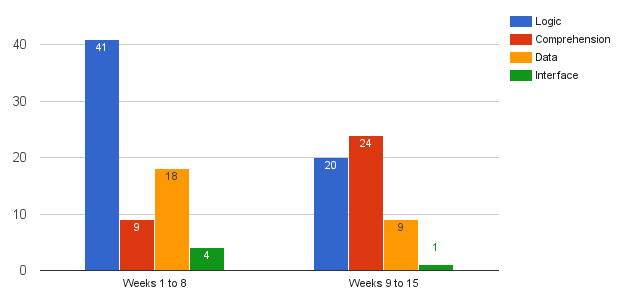
\includegraphics[scale=0.38]{figures/types.png}
\caption{Recorded bugs, split by type and time}
\label{fig:types}
\end{figure}
%-----------------------------------------------------------------


\newpage
Some bugs can be classified per the IEEE classification into logic,
data, or interface bugs when we look solely at the code. However, when
we take into account the student's reasoning behind the bug, we
realize that these are actually comprehension bugs. As mentioned in
Section \ref{sec:method}, six bugs that were initially classified as
logic or data bugs (per the IEEE standard) were later reclassified
as comprehension bugs. Figure \ref{fig:incorrect} is an example of a
bug that was reclassified.\\

Thus, while traditional bug taxonomies classify the bugs into
orthogonal categories based on a description of the bug (in code or
documentation) \cite{Beizer90}, our taxonomy requires additional
information about the student's reasoning in order to decide whether
or not a bug is a comprehension bug. This shows that when classifying
bugs in introductory computer science classes, it is not sufficient to
record just the bug itself. It is equally, if not more, important to
also record the student's understanding of the bug.\\

We were able to record \numtotal bugs throughout the course of the
semester. While it would have been ideal to be able to record a larger
number of bugs committed by students taking the class
\cite{BryceCooleyHansenHayrapetyan10}, we lacked the resources to
perform such widespread data collection.


%-----------------------------------------------------------------
\newpage
\section{Further Work}
%-----------------------------------------------------------------

It would be useful to collect a larger set of data about bugs seen in
class. One way to do this is to require students to complete a form
about their problem before and after receiving help at office hours
(where teaching assistants provide one-on-one help with programming
assignments). Not only would this give us a reliable and larger data
source, but it could also help improve the student and teaching
assistant experience at office hours. Firstly, requiring students to
document their problem before receiving help may discourage the often
vague and ill-defined questions that teaching assistants get about the
assignment, forcing students to think harder about the assignment
before asking for help. Secondly, asking students to include their
code in the report will allow the teaching assistants to download the
code on their own computer, which may help them diagnose the bug more
easily and correctly.\\

\newpage
Given our aim of using this taxonomy as a basis for a formal
discussion of bugs seen in the class, it is important to judge how
well a course staff can categorize bugs according to this taxonomy. We
are planning on conducting a study in Fall 2015 that asks teaching
assistants to categorize a random sample of bugs seen in the class.
This will help us fine-tune our taxonomy, and generate awareness of
this research among the course staff.\\

Consistent with our other aim of formulating plans to better prepare
students to deal with such errors, we now provide some suggestions on
how this research can help improve the quality of a class.\\

A system that would provide students hints about their errors, based
on their code and reasoning, can help students find and fix their bugs
more easily. Similarly, tutors have been developed for novice
programmers, which analyze student code to determine whether it
contains the appropriate algorithms and program components for a given
problem, and provide hints based on which components are missing or
incorrect \cite{Sudol-DeLyser14}. By taking into account student
reasoning, our proposed tutor may diagnose student error more
effectively.\\

An in-depth analysis of comprehension errors committed by students in
the class can help determine concepts that need to be explained better
in lectures.\\

Correlating student grades and performance with the bugs that they
commit may help us to predict the performance of individual students,
based on patterns from previous semesters.

%-----------------------------------------------------------------
\section{Conclusion}
%-----------------------------------------------------------------

In this paper, we aimed to take some first steps towards developing a
common basis and formal language for discussing bugs in introductory
computer science classes, which in turn will help instructors to
better prepare students to deal with such bugs when they arise. Our
approach was to document the bugs seen in an introductory computer
science class throughout the course of a semester. Our categorization
and analysis of those bugs showed that a category of bugs called
comprehension errors is prevalent in introductory computer science
classes. Since a comprehension error often highlights a concept that
was misunderstood by the student, such errors can provide useful
information on concepts that need to be explained better. Our
take-aways are a taxonomy of bugs that is generally applicable to
introductory computer science classes, and insights on how this
taxonomy can provide a basis for initiatives that will reduce the time
and effort that it takes to diagnose and fix these bugs.

\newpage
\bibliographystyle{abbrv}
\bibliography{mybib}
\balancecolumns

%-----------------------------------------------------------------
%-----------------------------------------------------------------
\end{document}
%-----------------------------------------------------------------
%-----------------------------------------------------------------
